%Kompilierung mit:
%latex -interaction=nonstopmode %.tex|bibtex %|dvipdfm %.dvi|"D:/Programme/Foxit Reader/Foxit Reader.exe" %.pdf

\documentclass[a4paper, 10pt]{article}
%\usepackage[utf8]{inputenc}			
\usepackage[german]{babel}		% for german	
\usepackage{graphicx}								
\usepackage{parskip}
\usepackage{listings}
\usepackage{xcolor}
\usepackage{amsmath}
\usepackage{mathtools}
\usepackage{amssymb}
\usepackage{titlesec}	
%\usepackage{tabularx}
%\usepackage{pdfpages}
%\usepackage{hyperref,breakurl}
%\usepackage{url}
%\usepackage{psfrag}
\usepackage{epstopdf}

\addtolength{\textwidth}{2.1cm}
\addtolength{\topmargin}{-1.4cm}
\addtolength{\oddsidemargin}{-1.1 cm}
\definecolor{leichtgrau}{gray}{0.91}
\setlength{\parindent}{0pt}

% \lstset{language = C,
	% basicstyle=\footnotesize,       
	% numbers=left,                  
	% numberstyle=\footnotesize,      
	% stepnumber=2,
	% numbersep=5pt,
	% backgroundcolor=\color{leichtgrau},
	% frame=single,
% }

% Definition von römischen Zahlen
\newcommand{\rom}[1]{$\underline{\overline{\text{#1}}}$} 


\begin{document}
\section{SIMO Systems}
\subsubsection*{Remarks}
\begin{itemize}
	\item In SIMO Systems only \underline{coding} and \underline{diversity} \underline{gains} can be exploited (no multiplexing gains)
	\item To realize these gains diversity combining has to be performed
	\item Diversity combining schemes vary in complexity and performance
	\item There are \underline{many} diversity combining schemes. Here we consider:
	\begin{itemize}
		\item Maximal ratio combining (MRC)
		\item Equal gain combining (EGC)
		\item Selection combining (SC)
	\end{itemize}
	\item Diversity combining problem
	\begin{figure}[h]\centering
		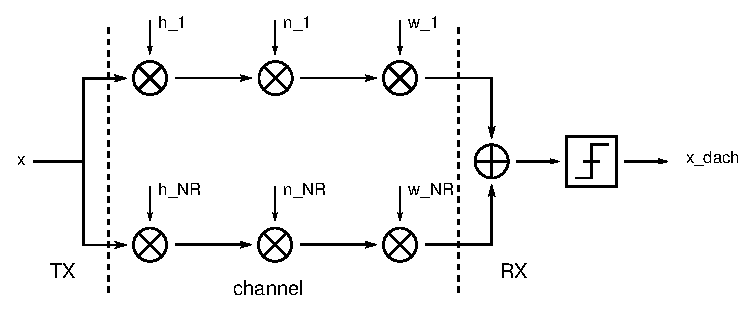
\includegraphics[width=0.8\textwidth]{Multi_Channel}
	\end{figure}		
	
	\begin{itemize}
		\item how to choose combining weights $w_n$?
		\item what performance (e.g. error rate, outage probability) is achieved?
		\item what \underline{diversity} and coding/combining gain is achieved?
	\end{itemize}
\end{itemize}
\begin{minipage}[hbt]{7cm}
	\centering
	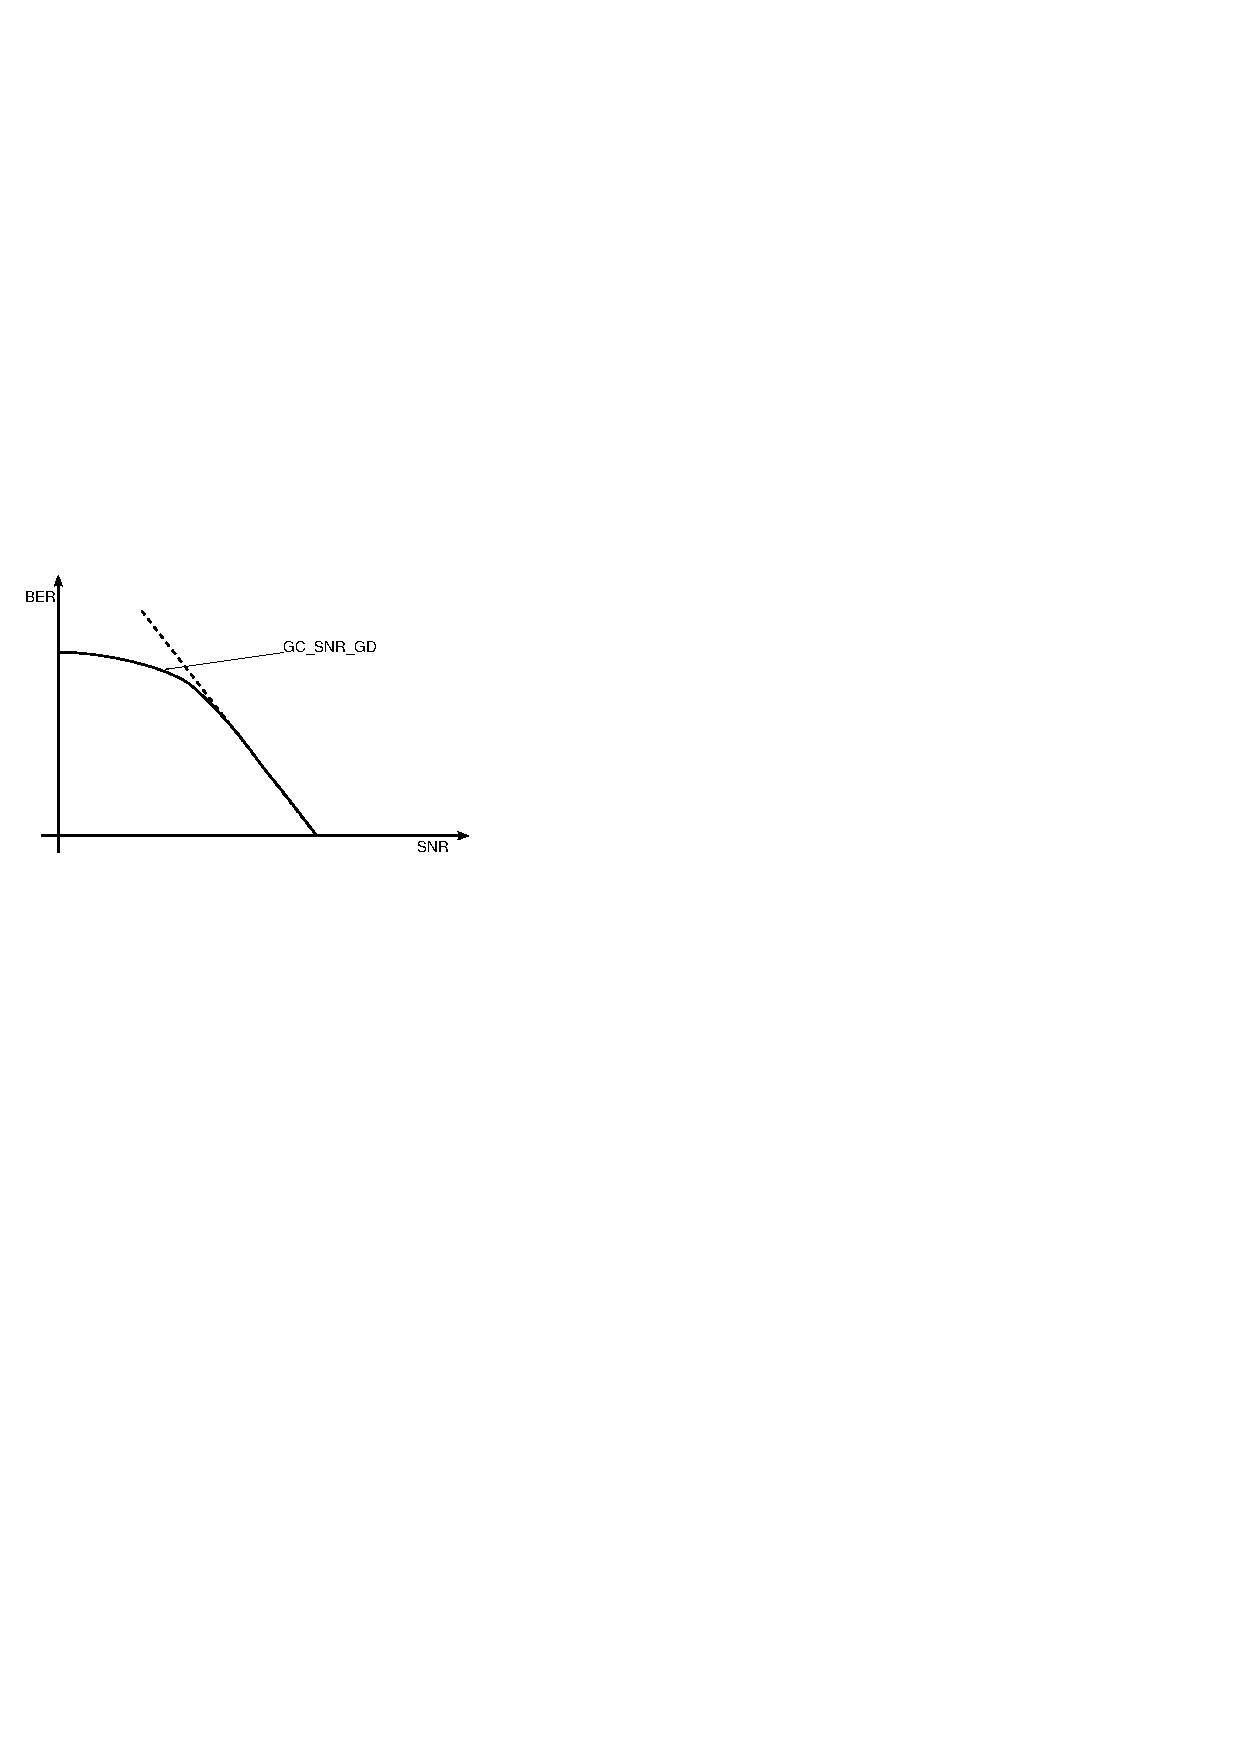
\includegraphics[width=7cm]{SIMO_BER_SNR_Kurve}
\end{minipage}
\hfill
\begin{minipage}[hbt]{5cm}
	\centering
		\begin{itemize}
			\item $G_c$ : Coding gain
			\item $G_d$ : Diversity gain
		\end{itemize}
\end{minipage}

\subsection{Preliminaries}
Consider an equivalent system:
\begin{align*}
	y &= hx +n;\\
	\mathcal{E}\{|x^2|\} &= \epsilon_s; & \mathcal{E}\{|n^2|\} &= \sigma_n^2; & \mathcal{E}\{|h|^2\} &= 1
\end{align*}
\begin{itemize}
	\item Instantaneous SNR: $\gamma_t = \frac{\epsilon_s}{\sigma_n^2}\times |h|^2$
\item Average SNR: $\bar{\gamma}_t = \mathcal{E}\{\gamma_t\} = \frac{\epsilon_s}{\sigma_n^2}$
\end{itemize}
\paragraph{Bit and Symbol Error Rate}
\begin{itemize}
	\item The Bit and Symbol Error Rate of many modulation schemes can be expressed for given $\gamma_t$ as:
\end{itemize}
\begin{align*}
	P_e(\gamma_t) = aQ\bigl\{ \sqrt{b\gamma_t}\bigr\}
\end{align*}
where:
\begin{itemize}
	\item $Q(x) = \frac{1}{\sqrt{2\pi}}\times\int_{x}^{\infty} e^{-\frac{t^2}{2}}~dt$
	\item $P_e(\gamma_t)$ may be exact result or approximation
	\item BPSK: exact with $a = 1, b = 2$
	\item M-ary QAM: tight approximation with $a = 4\bigl (1-\frac{1}{\sqrt{M}}\bigr ), b =  \frac{3}{M - 1}$
\end{itemize}
\begin{math} \bigl ({\small Einschub: Gray-Code: {BER} = \frac{1}{\log_2M} \times {SER} }\bigr ) \end{math}
\begin{itemize}
	\item Alternative representation of Q\;-\;function:
			\begin{align*} 
			Q(x) = \frac{1}{\pi}\int_{0}^{\frac{\pi}{2}} e^{-\frac{x^2}{2sin^2\theta}}~d\theta
			\end{align*}
			$\rightarrow$ Integral limits are fixed and do not depend on integration variables!
	\item Average error probability
		\begin{align*} 
		P_e = \mathcal{E}\bigl \{P_e(\gamma_t)\bigr \} = \int_{0}^{\infty}aQ\bigr (\sqrt{bx}\bigl )p_{\gamma_t}(x)~dx
		\end{align*}
		\begin{itemize}
			\item Integral may be difficult to solve analytically
			\item Integral has infinite support $\rightarrow$ numerical evaluation difficult
		\end{itemize}
	\item Using alternative representation of Q-function we get:
		\begin{align*}
			P_e &= \int_{0}^{\infty}\frac{a}{\pi}\int_{0}^{\frac{\pi}{2}}e^{-\frac{bx}{2sin^2\theta}}p_{\gamma_t}(x)~d\theta ~dx\\
			&= \frac{a}{\pi}\int_{0}^{\frac{\pi}{2}}\int_{0}^{\infty}p_{\gamma_t}(x)e^{-\frac{b}{2sin^2\theta}}~dx~d\theta &= \frac{a}{\pi}\int_{0}^{\frac{\pi}{2}}M_{\gamma_t}\bigl ( \frac{b}{2sin^2\theta} \bigr )~d\theta
		\end{align*}
where:
		\begin{itemize}
				\item $M_{\gamma_t}(s) = \int_{0}^{\infty}p_{\gamma_t}(x)e^{-sx}~dx$ is the Laplace transform of $p_{\gamma_t}$	
				\item $M_{\gamma_t}(-s)$ is the so called Moment Generation Function (MGF) of $p_{\gamma_t}$
				\item Here, we will also refer to $M_{\gamma_t}(s)$ as MGF
				\item $M_{\gamma_t}(s)$ is sometimes easier to obtain than $p_{\gamma_t}$
				\item The above integral can be easily evaluated numerically because of the finite integral limits
			\end{itemize}
\end{itemize}
\paragraph{Outage probability}
\begin{itemize}
	\item The outage probability is the probability that the channel cannot support a certain rate, R, i.e. (where \begin{math} \gamma_T \end{math} is the threshold SNR):
		\begin{align*}
			C = \log_2(1+\gamma_t) < R \quad \leftrightarrow \quad \gamma_t < 2^R - 1 \triangleq \gamma_T
		\end{align*}\\
		Thus, the outage probability is given by:
		\begin{align*}
			P_{out} &= P_0 {\gamma_t <\gamma-T}  \;= \int_{0}^{\gamma_T}p_{\gamma_t}(x)~dx
		\end{align*}
\item Using the inverse Laplace Transform\\
\begin{minipage}[hbt]{7cm}
	\centering
		\begin{align*}
			p_{\gamma  _t}(x) = \frac{1}{2\pi j}\int_{c-j\omega}^{c+j\omega}M_{\gamma _t}(s)e^{sx}~dx
		\end{align*}
	where \begin{math} c > 0\end{math} is a small constant that lies in the region of convergence of the integral, we obtain:
\end{minipage}
\hfill
\begin{minipage}[hbt]{5cm}
	\centering
	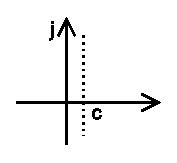
\includegraphics[width=2cm]{SIMO_Konstante_c}
\end{minipage}

\begin{itemize}
	\item 1.
			\begin{align*}
				P_{out} = \frac{1}{2\pi j}\int_{c-j\omega}^{c+j\omega}M_{\gamma _t}(s)\int_{0}^{\gamma _T}e^{sx}~dx~ds = \frac{1}{2\pi j}\int_{c-j\omega}^{c+j\omega}M_{\gamma _t}(s)e^{\gamma _Ts}~\frac{ds}{s}
			\end{align*}
			\begin{math}\bigl (\end{math}lower integral limit is 0 since \begin{math}p_{\gamma _t}(0) = 0 \bigr )\end{math}
	\item and 2.:
		\begin{align*}
			p_{\gamma _t} (x) &= \int_{0}^{x} p_{\gamma _t}(t) ~dt = 0\\		
		\text{for } x &= 0 \text{ note: } p_{\gamma _t}(x) \xleftrightarrow [transform]{Laplace} \frac{1}{s}M_{\gamma _t}(s)
		\end{align*}
	\end{itemize}
\end{itemize}
\paragraph{General combining scheme}
\begin{align*}
	y &= \Bigl (\sum_{n = 1}^{N_R}h_nw_n\Bigr )x + \sum_{n = 1}^{N_R}w_nn_n \\
	\gamma _t &= \frac{\epsilon _s \Bigl | \sum_{n = 1}^{N_R}h_nw_n\Bigr |^2 }{\sigma _n^2 \sum_{N = 1}^{N_R}|w_n|^2}
\end{align*}
where \begin{math} w_n\end{math} depends on the particular combining scheme.
\subsection{MRC (Maximum Ratio Combining)}
\begin{itemize}
	\item what weight \begin{math}w_n\end{math} maximize \begin{math}\gamma _t\end{math}?
	\begin{itemize}
		\item Cauchy-Schwarz inequality
		\begin{align*}
			\Bigl | \sum_{n = 1}^{N_R}h_nw_n\Bigr |^2 \leq \sum_{n = 1}^{N_R}|h_n|^2 \cdot \sum_{n = 1}^{N_R}|w_n|^2
		\end{align*}
	where equality holds if and only if \begin{math}w_n = c\cdot h_n^*\end{math} for some non-zero constant \begin{math}c\end{math}.
		\item for \begin{math}w_n = h_n^*\end{math}, we obtain
		\begin{align*}
			\gamma _t = \frac{\epsilon _s}{\sigma _n^2}\cdot \frac{\Bigl ( \sum_{n = 1}^{N_R}|h_n|^2\Bigr ) ^2}{\sum_{n = 1}^{N_R}|h_n|^2} = \frac{\epsilon _s}{\sigma _n^2}\sum_{n = 1}^{N_R}|h_n|^2
		\end{align*}
		\item \begin{math}w_n = h_n^* \forall n\end{math} are the MRC combining weights.	
	\end{itemize}
	\item For performance analysis we assume \underline{independent identically distributed (IID)} Rayleigh fading
		\begin{align*}
			\rightarrow \mathcal{E}\{|h_n|^2\} &= 1; \quad \bar{\gamma} = \frac{\epsilon _s}{\sigma	_n^2}; \quad \gamma _n = \frac{\epsilon _s}{\sigma _n^2}|h_n|^2\\
			p_{\gamma}(x) &= \frac{1}{\bar{\gamma}}e^{-\frac{x}{\bar{\gamma}}}; \quad x\geq 0\\
			M_{\gamma}(s) &= \frac{1}{1+s\bar{\gamma}}
		\end{align*}		
	\item Error rate
			\begin{align*}
				\gamma _t = \sum_{n = 1}^{N_R}\gamma _n
			\end{align*}
			\begin{math}\rightarrow \end{math} sum of IID random variables (r.v.s.)
			\begin{align*}
				M_{\gamma _t}(s) = \Bigl (M_\gamma (s)\Bigr )^{N_R} = \frac{1}{(1 + s\bar{\gamma})^{N_R}} = \frac{1}{\bar{\gamma}^{N_R}}\cdot \frac{1}{(s + \frac{1}{\bar{\gamma}})^{N_R}}
			\end{align*}
			inverse Laplace-transform (from tables)
			\begin{align*}
				p_{\gamma _t}(x) = \frac{1}{\bar{\gamma}^{N_R}}\cdot \frac{x^{N_R-1}}{(N_R - 1)!}e^{-\frac{x}{\bar{\gamma}}};\quad x\geq 0
			\end{align*}
	\item Direct approach 
		\begin{align*}
			p_e &= \int_{0}^{\infty}a\cdot Q\bigl (\sqrt{ax} \bigr )p_{\gamma _t}(x)~dx = a\Bigl (\frac{1 - \mu}{2}\Bigr )^{N_R} \cdot \sum_{n = 0}^{N_R - 1}\begin{pmatrix} N_R - 1 + n \\ n\end{pmatrix}\Bigl (\frac{1 + \mu}{2}\Bigr )^n \\ \text{where}\; \mu &= \sqrt{\frac{b\bar{\gamma}}{2 + b\bar{\gamma}}}
		\end{align*}
		\item MGF approach
			\begin{align*}
				p_e &= \frac{a}{\pi}\int_{0}^{\frac{\pi}{2}}M_{\gamma _t}\Bigl ( \frac{b}{2\sin ^2\theta}\Bigr )~d\theta \\
				&= \frac{a}{\pi}\int_{0}^{\frac{\pi}{2}}\frac{1}{\bar{\gamma}^{N_R}\bigl (\frac{b}{\sin ^2\theta} + \frac{1}{\bar{\gamma}}\bigr )^{N_R}}~d\theta \quad \text{(numerisch berechnen!)}
			\end{align*}
			\item high SNR: \quad \begin{math}\bar{\gamma}\rightarrow \infty \Longleftrightarrow \frac{1}{\bar{\gamma}}\rightarrow 0 \end{math}
	\begin{align*}
				p_e &= \frac{a}{\pi}\cdot\frac{1}{\bar{\gamma}^{N_R}}\cdot \Bigl (\frac{2}{b}\Bigr )^{N_R}\int_{0}^{\frac{\pi}{2}}\sin ^{2N_R}\theta ~d\theta \\
				 (\text{from MGF approach: }  &\int_{0}^{\frac{\pi}{2}}\sin ^{2N_R}\theta ~d\theta = \frac{\pi}{2^{N_R + 1}}\cdot \begin{pmatrix} 2N_R \\ N_R) \end{pmatrix}\\ &= \frac{a}{2^{N_R+1}\cdot b^{N_R}}\begin{pmatrix}2N_R & N_R\end{pmatrix}\frac{1}{\bar{\gamma}^{N_R}}\quad \text{as } \bar{\gamma} \rightarrow \infty \\ &\stackrel{!}{=} \Bigl (\frac{1}{G_c\bar{\gamma}}\Bigr )\\
				\text{where: Diversity gain: } & G_d = N_R\\	
				\text{Combining/Coding gain: } & G_c = 2b\Bigl (\frac{a}{2}\begin{pmatrix}2N_R \\ N_R\end{pmatrix}\Bigr )^{-\frac{1}{N_R}}	
	\end{align*}	
	\begin{figure}
		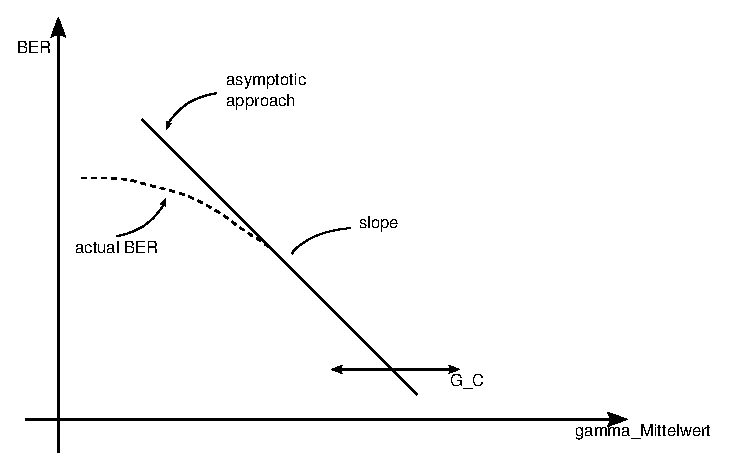
\includegraphics[width = 0.7\textwidth]{SIMO_BER_gamma_Kurve}
	\end{figure}
	\item MRC exploits the maximal possible diversity
	\item Diversity gain is not affected by correlation as the branches are not \underline{fully} correlated
	\item Diversity gain depends on fading distribution 
\end{itemize}
\paragraph*{Outage probability}
\begin{align*}
	P_{out} &= \int_{0}^{\gamma _T}p_{\gamma _t}(x)~dx = \frac{1}{\bar{\gamma}^{N_R}}\int_{0}^{\gamma _T}\frac{x^{N_R-1}}{(N_R - 1)!}e^{-\frac{x}{\bar{\gamma}}}~dx \\ &= 1- e^{-\frac{\gamma _T}{\bar{\gamma}}}\cdot \sum_{n = 1}^{N_R}\frac{\bigl (\frac{\gamma _T}{\bar{\gamma}}\bigr )^n}{(n - 1)!}
\end{align*}
\begin{itemize}
	\item Approximation (Taylor series): $\bar{\gamma}\rightarrow \infty : -e^{-\frac{x}{\bar{\gamma}}} = 1 - \frac{x}{\bar{\gamma}} + O(\frac{1}{\bar{\gamma}})$\; where a function $f(x) \text{ is } O(x) \text{ if } \lim\limits_{x\to\infty}\frac{f(x)}{x} = 0$.
\begin{align*}
	\Rightarrow P_{out}=\frac{1}{\gamma^{N_R}}\int\limits_0^{\gamma_T}\frac{x^{N_R-1}}{(N_R-1)!}\left(1-\frac{x}{\bar{\gamma}}+O\left(\frac{1}{\bar{\gamma}}\right)\right)
\end{align*}
	\item Diversity and coding gain can also be defined for $P_{out}$
\end{itemize}

\subsection{EGC (Equal Gain Combining)}

\paragraph*{Combining Weights}
\begin{itemize}
	\item For MRC, both, the amplitudes and phases of the channel gains $h_n=|h_n|e^{j\varphi_n}$ have to be known (or estimated in practice)
	\item In EGC it is assumed that only the phases are known and weights $w_n=e^{-j\varphi_n}$ are used.
\begin{align*}
	\Rightarrow \gamma_t &=\dfrac{\mathcal{E}_s}{\sigma_n^2}\dfrac{\left|\sum\limits_{n=1}^{N_R}|h_n|e^{j\varphi_n}e^{-j\varphi_n}\right|^2}{\sum\limits^{N_R}_{n=1}\left|e^{-j\varphi_n}\right|^2}
	=\frac{\mathcal{E}_s}{\sigma_n^2}\frac{1}{N_R}\left(\sum\limits^{N_R}_{n=1}|h_n|\right)^2\\
	&=\frac{1}{N_R}\left(\sum\limits_{n=1}^{N_R}\sqrt{\gamma_n}\right)^2;\text{  with  }\gamma_n=\frac{\mathcal{E}_s}{\sigma_n^2}|h_n|^2
\end{align*}
\end{itemize}
\paragraph*{Performance Analysis}
\begin{itemize}
	\item i.i.d. case \\
	$\Rightarrow$ $\sqrt{\gamma_n}$ is Rayleigh distributed\\
	$\Rightarrow$ Exact analysis is much more difficult than for MRC $\Rightarrow$ see book by Simon\;\&\;Alouini p.341
	\item Approximate result
\begin{align*}
	P_e=\frac{a}{2}\left[1-\sqrt{\frac{2b\bar{\gamma}}{5+2b\bar{\gamma}}}\sum\limits_{n=0}^{N_R-1}\frac{\left(\! \begin{array}{c} 2n \\ n \end{array} \!\right) }{4^n(1+\frac{2}{5}b\bar{\gamma})^n}\right]
\end{align*}
	\item high SNR\\
	$\Rightarrow$ use high SNR analysis of Wang\;\&\;Giannakis, 2003\\
	$\Rightarrow$ at high SNR, only pdf of $\gamma_n$ around $0$ is relevant for performance
\begin{align*}
	\Rightarrow \overset{\text{Rayleigh}}{p_\gamma(x)} = \frac{1}{\bar{\gamma}}e^{-\frac{x}{\bar{\gamma}}}\overset{\text{Taylor Serie}}{=}\frac{1}{\bar{\gamma}}+O\left(\frac{1}{\bar{\gamma}}\right)\text{ as } x \to 0
\end{align*}
	\item need pdf $\gamma _t$: ($\gamma _n$ bekannt, $\rightarrow$ ges.: Wurzel, etc.)\\ (cumulative distribution function of $\sqrt{\gamma}\;(\overset{\text{i.i.d}}{=}\sqrt{\gamma_n}) $ (cdf))
	\begin{align*}
	% 1. Formel
		P_{\sqrt{\gamma}}(x) &= Pr\bigl\{\sqrt{\gamma}\leq x \bigr\} =  Pr\bigl\{\gamma\leq x^2 \bigr\} = P_{\gamma}(x^2) = \text{cdf of}\;\gamma\\
	% 2. Formel
		\rightarrow p_{\sqrt{\gamma}}(x) &= \frac{d}{dx}P_{\sqrt{\gamma}}(x) = 2x\cdot p_{\gamma}(x^2) = \frac{2x}{\bar{\gamma}} + O\bigl(\frac{1}{\bar{\gamma}}\bigr)\\
	\end{align*}
	\item Laplace Transformation to MGF
	\begin{align*}
	% 3. Formel
		\rightarrow M_{\sqrt{\gamma}}(s) &= \mathcal{L}\bigl\{p_{\sqrt{\gamma}}(x)\bigr\} = \frac{2}{\bar{\gamma}}\cdot \frac{1}{s^2} + O\bigl(\frac{1}{\bar{\gamma}}\bigr)\\
	% 4. Formel
		\sqrt{\gamma _t} &= \sum_{n = 1}^{N_R}\frac{\sqrt{\gamma _n}}{N_R}\\
	% 5. Formel
		 M_{\sqrt{\gamma _t}}(s) &= \mathcal{E}\Bigl\{\mathrm{exp}({-s\sqrt{\gamma _t}})\Bigr\} = \mathcal{E}\Bigl\{\mathrm{exp}({-\frac{s}{\sqrt{N_R}}\cdot \sum_{n = 1}^{N_R}\sqrt{\gamma _n}})\Bigr\} = \Bigl(\mathcal{E}\Bigl\{\mathrm{exp}(-\frac{s}{\sqrt{N_R}}\cdot \sqrt{\gamma _n}\Bigr\}\Bigr)^{N_R}\\
	% 6. Formel
		 &= \Bigl( M_{\sqrt{\gamma}}\bigl(\frac{s}{\sqrt{N_R}}\bigr) \Bigr)^{N_R} = \Bigl(\frac{2}{\bar{\gamma}}\cdot \frac{N_R}{s^2}\Bigr)^{N_R} + O\Bigl(\frac{1}{\bar{\gamma}^{N_R}}\Bigr)\\
	\end{align*}
	\item inverse Laplace Transform
	\begin{align*}
	% 7. Formel
		p_{\sqrt{\gamma _t}}(x) &= \mathcal{L} ^{-1}\Bigl\{M_{\sqrt{\gamma _t}}(s)\Bigr\} = \Bigl(\frac{2N_R}{\bar{\gamma}}\Bigr)^{N_R}\cdot \frac{x^{2N_R-1}}{(2N_R-1)!} + O\Bigl(	\frac{1}{\bar{\gamma}^{N_R}}\Bigr)\\
	% 8. Formel
		P_{\gamma _t}(x) &= Pr\bigl\{\gamma _t\leq x	\bigr\} =  Pr\bigl\{\sqrt{\gamma _t}\leq \sqrt{x}\bigr\} = P_{\sqrt\gamma _t}(\sqrt{x}) \rightarrow \text{cdf of } \sqrt{\gamma _t}\\
	% 9. Formel
		p_{\gamma _t}(x) &= \frac{d}{dx}P_{\gamma _t}(x) = \frac{1}{2\sqrt{x}}\cdot p_{\gamma _t}(\sqrt{x}) = \frac{1}{2}\Bigl(\frac{2N_R}{\bar{\gamma}} \Bigr)^{N_R}\cdot \frac{x^{N_R-1}}{(2N_R-1)!} + O\bigl(\bar{\gamma}^{-N_R}\bigr)\\
	% 10. Formel
		\rightarrow M_{\gamma _t}(s) &= \mathcal{L}\bigl\{p_{\gamma _t}(x)\bigr\} = \frac{1}{2}\Bigl( \frac{2N_R}{\bar{\gamma}}\Bigr)^{N_R}\cdot \frac{(N_R - 1)!}{(2N_R -1)!~b^{N_R}} + O\bigl(\bar{\gamma}^{-N_R}\bigr)\\
	% 11. Formel
	\end{align*}
	\item Error Probability:
\begin{align*}
        P_e&=\frac{a}{\pi}\int\limits_0^{\frac{\pi}{2}}M_{\gamma_t}\left(\frac{b}{2\sin^2(\theta)}\right)\mathrm{d}\theta\\
        &=\frac{a}{\pi}\frac{1}{2}\left(\frac{2N_R}{\bar{\gamma}}\right)^{N_R}\frac{(N_R-1)!}{(2N_R-1)!}
        \frac{2^{N_R}}{b^{N_R}}
        \underbrace{\int\limits_0^{\frac{\pi}{2}}\sin^{2N_R}(\theta)\mathrm{d}\theta}_
        {\frac{\pi}{2^{2N_R+1}}\binom{2N_R}{N_R}=\frac{\pi(2N_R)!}{2^{2N_R+1}(N_R!)^2}}
        +O\left(\frac{1}{\bar{\gamma}^{N_R}}\right)\\
        &= \frac{aN_R^{N_R}}{2b^{N_R}N_R!}\frac{1}{\bar{\gamma}^{N_R}}+O\left(\frac{1}{\bar{\gamma}^{N_R}}\right)
        \overset{!}{=}\left(\frac{1}{G_c}\right)^{G_d}
\end{align*}

\begin{itemize}
		\item[] $\Longrightarrow \text{Diversity gain: } G_d = N_R$
		\item[] $\Longrightarrow \text{Combining gain: } G_c = \frac{b}{N_R}\Bigl( \frac{2N_R!}{a}\Bigr)^{\frac{1}{N_R}}$
		\item[] vergleiche auch Blatt mit Kurven \rom{III} und \rom{IV}
	\end{itemize}
\end{itemize}
A similar asymptotic analysis can be conducted for the outage probability.
\subsection{SC (Selection Combining)}
\paragraph*{Combining weights}
	\begin{itemize}
		\item only the strongest branch is chosen
		\item strongest branch: $\hat{n} = \underset{n}{\text{argmax}} \gamma _n \longrightarrow \gamma _t = \gamma _{\hat{n}}$
		\item only on RF receiver chain required $\rightarrow$\; saves hardware complexity 
	\end{itemize}
\paragraph*{Performance analysis}
	\begin{itemize}
		\item cdf of: $\gamma _t$
			\begin{align*}
				P_{\gamma _t}(x) &= Pr\bigl\{\gamma _{\hat{n}} \leq x\bigr\} = Pr\bigl\{\gamma _1 \leq x \cap \gamma _2 \leq x \cap \dots \gamma _{N_R} \leq x\bigr\}\\
				&\overset{(IID)}{=} \Bigl(Pr\bigl\{\gamma _n \leq x\bigr\}\Bigr)^{N_R} = \Bigl( P_{\gamma}(x)\Bigr)^{N_R}
			\end{align*}
		\item pdf:
			\begin{align*}
				p_{\gamma _t}(x) &= \frac{d}{dx}P_{\gamma _t}(x) = N_R\bigl(P_{\gamma}(x)\bigr)^{N_R-1}\cdot p_{\gamma}(x)\\
				\text{where: }\qquad p_{\gamma _t}(x) &= \frac{1}{\bar{\gamma}}e^{-\frac{x}{\bar{\gamma}}};\quad x\geq 0\\
				P_{\gamma}(x) &= \int_{0}^{x}p_{\gamma}8x)~dx = 1 - e^{-\frac{x}{\bar{\gamma}}};\quad x\geq 0\\
				\rightarrow p_{\gamma _t}(x) &= \frac{N_R}{\bar{\gamma}}\bigl( 1 - e^{-\frac{x}{\bar{\gamma}}}\bigr)^{N_R-1}e^{-\frac{x}{\bar{\gamma}}};\quad x\geq 0
			\end{align*}
	\end{itemize}
\paragraph*{Error probability}
	\begin{itemize}
		\item direct approach $\rightarrow$ closed-form solution possible
		\item MGF approach
		\begin{itemize}
			\item Binomial expansion\\
			\begin{align*}
				p_{\gamma _t}(x) &= \frac{N_R}{\bar{\gamma}}e^{-\frac{x}{\bar{\gamma}}}\sum_{n = 0}^{N_R - 1}\begin{pmatrix} N_R - 1 \\ n\end{pmatrix} 1^{N_R - 1 - n}\Bigl( -e^{-\frac{x}{\bar{\gamma}}}\Bigr)^n \\
				&= \frac{N_R}{\bar{\gamma}}\sum_{n = 0}^{N_R - 1}\begin{pmatrix}N_R - 1 \\ n\end{pmatrix}\cdot (-1)^{n}e^{-\frac{x(n + 1)}{\bar{\gamma}}};\quad	x \geq 0
			\end{align*}
			\item MGF\\
			\begin{align*}
				M_{\gamma _t}(s) = \frac{N_R}{\bar{\gamma}}\sum_{n = 0}^{N_R - 1}\begin{pmatrix}N_R - 1\\n\end{pmatrix}(-1)^{n}\frac{1}{s + \frac{n+1}{\bar{\gamma}}}
			\end{align*}
			\item 
			\begin{align*}
				P_e = \frac{a}{\pi}\int_{0}^{\frac{\pi}{2}}M_{\gamma _t}\Bigl(\frac{b}{2\sin^2\theta}\Bigr)~d\theta = \frac{aN_R}{\pi\bar{\gamma}}\sum_{n = 0}^{N_R - 1}\begin{pmatrix}N_R - 1\\ n\end{pmatrix} (-1)^{n}\int_{0}^{\frac{\pi}{2}}\frac{d\theta}{\frac{b}{2\sin^2\theta} + \frac{n + 1}{\bar{\gamma}}}\\ \rightarrow\text{can be evaluated numerically}				
			\end{align*}
		\end{itemize}
	\end{itemize}

\end{document}
